\documentclass[10pt,nofootinbib]{revtex4}
\usepackage{amsmath,amssymb,amsfonts,mathrsfs,bm,dsfont}
\usepackage[all]{xy}
\usepackage[normalem]{ulem}	% delete line
\usepackage{graphics,color}
\usepackage{tikz}
	\usetikzlibrary{calc}
	\usetikzlibrary{decorations.markings}
	\usetikzlibrary{arrows}
\usepackage{pgfplots}


%\usepackage{hyperref}
\usepackage{feynmp} % feymann diagram
\usepackage{extarrows}


\newcommand*\dd{\mathop{}\!\mathrm{d}}
\newcounter{Claim}[section]
\newenvironment{Claim}[1][]{{\par\normalfont\bfseries \underline{Claim~\stepcounter{Claim}\arabic{Claim}.}~#1~~}}{\par}
\newcounter{Proposition}[section]
\newenvironment{Proposition}[1][]{{\par\normalfont\bfseries \underline{Proposition~\stepcounter{Proposition}\arabic{Proposition}.}~#1~~}}{\par}
\newcounter{Note}[section]
\newenvironment{Note}[1][]{{\par\normalfont\bfseries \underline{Note~\stepcounter{Note}\arabic{Note}.}~#1~~}}{\par}
\newcounter{Lemma}[section]
\newenvironment{Lemma}[1][]{{\par\normalfont\bfseries \underline{Lemma~\stepcounter{Lemma}\arabic{Lemma}.}~#1~~}}{\par}
\newcounter{Corollary}[section]
\newenvironment{Corollary}[1][]{{\par\normalfont\bfseries \underline{Corollary~\stepcounter{Corollary}\arabic{Corollary}.}~#1~~}}{\par}
\newenvironment{Proof}{{\par~{\normalfont\bfseries $\vartriangleright$}~~}}{\hfill $\square$\par\hfill\par} %\par
\newcounter{Def}[section]
\newenvironment{Def}[1][]{{\par\normalfont\bfseries \underline{Definition~\stepcounter{Def}\arabic{Def}.}~#1~~}}{\par}

\allowdisplaybreaks[4] %允许 align 跨页编排

\def\Re{\mathop{\mathcal{R}e}}
\def\Im{\mathop{\mathcal{I}m}}
\def\imp{\text{imp}}

\def\arrow{\tikz[scale=0.1,baseline=.1ex]{
	\draw[fill=black,rotate=-90] (-0.7,0)--(0,2)--(0.7,0);}
	}

\def\cross{\tikz[scale=0.1,baseline=.1ex]{
	\draw[thick,rotate=45] (-1,0)--(1,0);
	\draw[thick,rotate=45] (0,-1)--(0,1);}
	}





\begin{document}
\title{Kondo Effect and Kondo Problem}% Force line breaks with \\
%\thanks{This is a reminiscent note for Hubbard-Stratonovich Transformation.}%

\author{Xiaodong Hu}
%\altaffiliation[Also at ]{Boson College}
\email{xiaodong.hu@bc.edu}
\affiliation{Department of Physics, Boston College}

\date{\today}


\begin{abstract}
	This is a pedagogical review of the Kondo effect and Kondo problem. Calculation details of Schrieffer-Wolff transformation, spin scattering processes and RG analysis are recovered. Personal comments are also recorded.
\end{abstract}
\maketitle
\tableofcontents

\begin{fmffile}{hxd} % Documents containing feynmann diagrams
      \fmfcmd{%
        vardef cross_bar (expr p, len, ang) =
          ((-len/2,0)--(len/2,0))
          rotated (ang + angle direction length(p)/2 of p)
          shifted point 0 of p shifted (0,1.5mm)
        enddef;
        style_def crossed expr p =
          cdraw (wiggly p);
          ccutdraw cross_bar (p, 3mm, 45);
          ccutdraw cross_bar (p, 3mm, -45);
          cdraw fullcircle scaled 3mm shifted point 0 of p shifted (0,1.5mm);
        enddef;}
\iffalse
\section{Experimental Results}
	\subsection{Minimum of Resistance}
		
	\subsection{Phase out of Kondo Term}
	\subsection{Constant Magnetic Susceptibility}
	\subsection{Non-Fermi Liquid Behavior}
\fi
\section{Effective Hamiltonian}
	\subsection{Impurities in Mott Insulator: Anderson Model} 
		Anderson proposed his model
		\begin{align}
			H&=H_f+H_d+H_{\text{correlation}}+H_{\text{hybrid}},\nonumber\\
			&=\sum_{k \sigma}\varepsilon_kc_{k\sigma}^\dagger c_{k\sigma}+\sum_{\sigma}\varepsilon_d d_{\sigma}^\dagger d_{\sigma}+Un_{d\uparrow}n_{d\downarrow}+\sum_{k\sigma}V_k\big(c_{k\sigma}^\dagger d_{\sigma}+h.c.\big)\label{1.1.1}
		\end{align}
		in study of localized moments early in \cite{anderson1961localized}. This is an appropriate description of \emph{localized and magnetic} d-state  impurities and s-state \emph{free} itinerate electrons because mean field study exhibits a magnetic phase for impurities, which is demanded for experimental observations.

	\subsection{Schrieffer-Wolff Transformation to Single-occupied Effective Hamiltonian}
		But mean-field (or Hartree-Fock) methods fails to grab the correct low-energy effective physics for such a strongly-correlation system. If we narrow our discussion to the effect of single impurity, then like the case in Heisenberg model, \emph{superexchange mechanism} occurs at \emph{half-filling} and \emph{large-U limit} \cite{Fradkin2013Field,altland2010condensed}. But there is no confinement on the number of occupation in origianl Anderson model, so certainly we need to develop a new method, projecting out the unphysical empty and doubly occupied Hilbert space to find out the proper effective Hamiltonian for Kondo physics. And Schrieffer-Wolff transformation \cite{schrieffer1966relation} is the standard technique.\par
		First of all, we can re-arrange original Anderson Hamiltonian by the number of impurity occupation
		\begin{equation*}
			H_{ij}\equiv P_iHP_j,
		\end{equation*}
		where $P_2=n_{d\uparrow}n_{d\downarrow}, P_1=n_{d\uparrow}(1-n_{d\downarrow})+n_{d\downarrow}(1-n_{d\uparrow})$, and $P_0=\mathds{1}-P_1-P_2$. Fortunate enough, without cumbersome commutator calculations, for \eqref{1.1.1} without hybridized term we can just substitute the number of impurities, obtaining
		\begin{subequations}
			\begin{align}
				H_{00}&\equiv P_0HP_0=\sum_{k \sigma}\varepsilon_{k}c_{k\sigma}^\dagger c_{k\sigma},\label{1.2.1a}\\
				H_{11}&\equiv P_1HP_1=\sum_{k \sigma}\varepsilon_{k}c_{k\sigma}^\dagger c_{k\sigma}+\varepsilon_d,\label{1.2.1b}\\
				H_{22}&\equiv P_2HP_2=\sum_{k \sigma}\varepsilon_{k}c_{k\sigma}^\dagger c_{k\sigma}+2 \varepsilon_d+U,\label{1.2.1c}
			\end{align}
		\end{subequations}
		while for the contribution from hybridized term,
		\begin{subequations}
			\begin{align}
				H_{01}&\equiv P_0HP_1=\sum_{k\sigma}V_kc_{k\sigma}^\dagger d_\sigma n_{d\sigma}(1-n_{d\bar{\sigma}})\label{1.2.2a}\\
				H_{12}&\equiv P_1HP_2=\sum_{k\sigma}V_kc_{k\sigma}^\dagger d_\sigma n_{d\sigma}n_{d\bar{\sigma}}\label{1.2.2b}\\
				H_{02}&\equiv P_0HP_2=0\label{1.2.2c}.
			\end{align}
		\end{subequations}
		The last term vanishes because hybridization term only involves single-particle creation and annihilation procedure. So in the basis of $\{P_0|\psi\rangle,P_1|\psi\rangle,P_2|\psi\rangle\}$, Anderson Hamiltonian can splitted by blocks
		\begin{equation}\label{1.2.3}
			H=\left(\begin{array}{ccc}
				H_{00}&H_{01}&0\\H_{10}&H_{11}&H_{12}\\0&H_{21}&H_{22}
			\end{array}\right).
		\end{equation}
		Treating the off-diagnal terms as pertubation (because tunnelings between subspcaces with distinct number of occupation is extremely suppressed by large-U limit), then our task is to diagonalize \eqref{1.2.3} and project out empty and doubly occupied degree of freedoms.\par
		Instead of considering the original Hamiltonian $H\equiv H_0+V$, where in our problem, $H_0\equiv\mathrm{\mathop{diag}}(H_{00},H_{11},H_{22})$ and 
		\begin{equation*}
			V\equiv\left(\begin{array}{ccc}
				0&H_{01}&0\\H_{10}&0&H_{02}\\0&H_{20}&0
			\end{array}\right),
		\end{equation*}
		we try to find a canonical transformation
		\begin{align}
			\widetilde{H}\equiv e^{S}He^{-S}&=H+[S,H]+\dfrac{1}{2!}[S,[S,H]]+\cdots\nonumber\\
			&=H_0+V+[S,H_0]+[S,V]+\dfrac{1}{2!}[S,[S,H_0+V]]+\cdots\label{1.2.4}
		\end{align}
		such that
		\begin{equation}\label{1.2.5}
			V+[S,H_0]\equiv0,
		\end{equation}
		where to keep the unitarity $S\equiv-S^\dagger$. Then up to the second order we are left with
		\begin{equation}\label{1.2.6}
			\widetilde{H}^{(2)}=H_0+[S,V]+\dfrac{1}{2}[S,[S,H_0]]=H_0+\dfrac{1}{2}[S,H_0].
		\end{equation}

		What we have done is to \textbf{\color{red}rearrange the perturbation series so that the odd-time transition (which is suppressed by large-U limit) is moved behind the even-time transition (which keep the number of occupation), and the abrupt truncation is able to tell us the correct low-energy physics for \emph{gapped system} (this procedure can also be understood in the sense of renormalization).}\footnote{Thanks to the online discussion with Ju-Ge Li, see \url{https://www.zhihu.com/question/272140639/answer/366066720}.}\par
		Schrieffer and Wolff \emph{Ansatzed} the form of canonical transformation in their original work \cite{schrieffer1966relation} through observation, whose coefficients can determined by requirement \eqref{1.2.5}. Lengthy calculation details are recoverd in \cite{phillips2012advanced}. Here, instead, we try to give a systematic way to solve $S$. This exploration is valuable demonstrating the equivalence of different approaches obtaining the effective Hamiltonian and can be easily generalized for other strongly-correlated spin system in future research.\par

		Noting the fact that any form of matrics should keep the form after commuting with an diagonal matrics. So from equation \eqref{1.2.5} we can write
		\begin{equation*}
			S=\left(\begin{array}{ccc}
				0&s_1&0\\-s_1^\dagger&0&s_2\\0&-s_2^\dagger&0
			\end{array}\right),
		\end{equation*}
		giving two indepent equations (note that each component of $S$ is still an many-body operator)
		\begin{subequations}
			\begin{align}
				s_1H_{11}-H_{00}s_1&=H_{01}\label{1.2.7a}\\
				s_2H_{11}-H_{22}s_2&=H_{12}\label{1.2.7b}
			\end{align}
		\end{subequations}
		Operator equations \eqref{1.2.7a} and \eqref{1.2.7b} are hard to solve unless we acting them on some many-body states. Suppose many-body state has energy $E$, i.e., $H|\psi\rangle=E|\psi\rangle$, then acting \eqref{1.2.7a} and \eqref{1.2.7b} on $|\psi_1\rangle\equiv P_1|\psi\rangle$, respectively, we have
		\begin{equation}\label{1.2.8}
			s_1=-\dfrac{1}{E-H_{00}}H_{01},\quad s_2=-H_{12}\dfrac{1}{H_{22}-E}.
		\end{equation}
		So the effective Hamiltonian (up two second order, in single-occupied subspace) is
		\begin{align}
			H^{(2)}_{\text{eff}}&\equiv P_1\left(H_0+\dfrac{1}{2}[S,V]\right)P_1\nonumber\\
			&=P_1\left\{H_0+\dfrac{1}{2}\left(\begin{array}{ccc}
				s_1H_{10}-H_{01}s_1^\dagger&0&s_1H_{12}+H_{01}s_2\\
				0&-s_1^\dagger H_{01}-H_{10}s_1+s_2H_{21}+H_{12}s_2^\dagger&0\\
				-s_2^\dagger H_{01}-H_{21}s_2^\dagger&0&-s_2^\dagger H_{12}+H_{12}s_2
			\end{array}\right) \right\}P_1\nonumber\\
			&=H_{11}+H_{10}\dfrac{1}{E-H_{00}}H_{01}+H_{12}\dfrac{1}{E-H_{22}}H_{21},\label{1.2.9}
		\end{align}
		or more explicitly %(for single-occupied subspace $n_{d\sigma}\equiv 1$ for whatever $\sigma=\uparrow,\downarrow$)
		\begin{align}
			H_{\text{eff}}^{(2)}&=\sum_{k}\varepsilon_k c_{k\sigma}^\dagger c_{k\sigma}\nonumber\\
			&+\sum_{kk'\sigma\sigma'}V_k^*V_{k'}\left((1-n_{d\bar{\sigma}})n_{d\sigma}d_\sigma c_{k\sigma}\dfrac{1}{E-H_{00}}c_{k'\sigma'}^\dagger d_{\sigma'}^\dagger n_{d\sigma'}(1-n_{d\bar{\sigma'}})+d_\sigma n_{d\sigma}n_{d\bar{\sigma}}c_{k\sigma}^\dagger\dfrac{1}{E-H_{22}}c_{k'\sigma'}n_{d\bar{\sigma'}}n_{d\sigma'}d_{\sigma'}^\dagger \right).\label{1.2.10}
		\end{align}
		\indent To prepare for further practicable calculation of spin Hamiltonian, perturbation and truncation on the free Green operator $G_{00}\equiv1/(E-H_{00})$ and $G_{22}\equiv1/(E-H_{22})$ must be performed. Since
		\begin{align*}
			H_{00}^nc_{k \sigma}^\dagger&\equiv\left(\sum_{p\mu}\varepsilon_p c_{p \mu}^\dagger c_{p\mu}\right)^n c_{k \sigma}^\dagger=\left(\sum_{p\mu}\varepsilon_p c_{p \mu}^\dagger c_{p\mu}\right)^{n-1}\sum_{p \sigma}\varepsilon_p c_{p\mu}^\dagger(\delta_{\mu\sigma}\delta_{p,k}-c_{k \sigma}^\dagger c_{p\mu})\\
			&=\left(\sum_{p\mu}c_{p \mu}^\dagger c_{p\mu}\right)^{n-1}c_{k\sigma}^\dagger\left(\varepsilon_k+\sum_{p \sigma}c_{p\mu}^\dagger c_{p\sigma}\right)=\cdots=c_{k\sigma}^\dagger\left({\color{red}\varepsilon_k}+\sum_{p \sigma}c_{p\mu}^\dagger c_{p\sigma}\right)^n,
		\end{align*}
		and similarly
		\begin{equation*}
			H_{22}^n c_{k \sigma}\equiv\left(\sum_{p\mu}\varepsilon_p c_{p\mu}^\dagger c_{p\mu}+2\varepsilon_d+U\right)^nc_{k\sigma}=\left({\color{red}-\varepsilon_k}+\sum_{p\mu}\varepsilon_p c_{p\mu}^\dagger c_{p\mu}+2 \varepsilon_d+U\right)^n,
		\end{equation*}
		terms in \eqref{1.2.9} containing Green operators can be simplified as
		\begin{align*}
			\dfrac{1}{E-H_{00}}c_{k\sigma}^\dagger&\equiv\dfrac{1}{E}\left(1-\dfrac{H_{00}}{E}\right)^{-1}c_{k\sigma}^\dagger=\dfrac{1}{E}\sum_{n=0}^\infty\dfrac{H_{00}^n}{E^n}c_{k\sigma}^\dagger=\dfrac{c_{k\sigma}^\dagger}{E}\sum_{n=0}^\infty\dfrac{(\varepsilon_k+H_{00})^n}{E^n}=\dfrac{c_{k\sigma}^\dagger}{E}\dfrac{1}{1-\dfrac{\varepsilon_k+H_{00}}{E}}\\
			&=c_{k \sigma}^\dagger\dfrac{1}{E-H_{00}-\varepsilon_k}\equiv c_{k \sigma}^\dagger\dfrac{1}{E-H_{11}-\varepsilon_k+\varepsilon_d}=\dfrac{c_{k \sigma}^\dagger}{\varepsilon_d- \varepsilon_k}\left(1+\dfrac{E-H_{11}}{\varepsilon_d- \varepsilon_k}\right)^{-1}\\
			&\simeq\dfrac{c_{k \sigma}^\dagger}{\varepsilon_d- \varepsilon_k}+\mathcal{O}(|E-H_{11}|^2),
		\end{align*}
		and similarly
		\begin{align*}
			\dfrac{1}{E-H_{22}}c_{k\sigma}&=c_{k \sigma}\dfrac{1}{E-H_{22}+\varepsilon_k}\equiv c_{k \sigma}\dfrac{1}{E-H_{11}+\varepsilon_k-\varepsilon_d-U}=\dfrac{c_{k \sigma}}{\varepsilon_k-U- \varepsilon_d}\left(1+\dfrac{E-H_{11}}{\varepsilon_k-U- \varepsilon_d}\right)^{-1}\\
			&\simeq\dfrac{c_{k \sigma}}{\varepsilon_k-U- \varepsilon_d}+\mathcal{O}(|E-H_{11}|^2),
		\end{align*}
		where we replace $H_{00}$ and $H_{22}$ with $H_{11}$ because by our construction $H_{11}$ dominant the contribution of eigen-energy $E$ because empty and doubly occupied configurations are highly suppressed. Therefore, we come to the final expression of the effective Hamiltonian up to the second order approximation for single-occupied configurations
		\begin{align}
			H_{\text{eff}}^{(2)}&=\sum_{k \sigma}\varepsilon_k c_{k \sigma}^\dagger c_{k \sigma}+\sum_{kk' \sigma\sigma'}V_k^*V_{k'}\left(\dfrac{(1-n_{d\bar{\sigma}})n_{d\sigma}d_\sigma^\dagger d_{\sigma'}n_{d\sigma'}(1-n_{d\bar{\sigma'}})}{\varepsilon_d- \varepsilon_{k'}}c_{k \sigma}c_{k'\sigma'}^\dagger+\dfrac{d_\sigma n_{d\bar{\sigma}}n_{d\sigma}n_{d\sigma'} n_{d\bar{\sigma'}}d_{\sigma'}^\dagger}{U+\varepsilon_d- \varepsilon_{k'}}c_{k \sigma}^\dagger c_{k'\sigma'}\right)\nonumber\\
			&=\sum_{k \sigma}\varepsilon_k c_{k \sigma}^\dagger c_{k \sigma}+\sum_{kk' \sigma\sigma'}V_k^*V_{k'}\left(\dfrac{d_\sigma^\dagger d_{\sigma'}}{\varepsilon_d- \varepsilon_{k'}}c_{k \sigma}c_{k'\sigma'}^\dagger+\dfrac{d_\sigma d_{\sigma'}^\dagger}{U+\varepsilon_d- \varepsilon_{k'}}c_{k \sigma}^\dagger c_{k'\sigma'}\right),\label{1.2.11}
		\end{align}
		where in the second line we implement the single-occupied condition so that the only non-vanishing term for each part is equivalent to those dropping all terms containing particle numbers.
	\subsection{Spin Hamiltonian: sd Model}
		We will see in this section that spacial degree of freedom in effective Hamiltonian \eqref{1.2.11} is actually projected out. So we should end up with a spin Hamiltonian. Introducing the spin operator for free electrons and impurities in the language of second quantization,
		\begin{equation*}
			\bm{S}_{kk'}\equiv\sum_{\alpha \beta}c_{k \alpha}^\dagger\dfrac{\bm{\sigma}_{\alpha \beta}}{2}c_{k \beta},\quad\bm{S}_d\equiv\sum_{\mu\nu}d_\mu^\dagger\dfrac{\bm{\sigma}_{\mu\nu}}{2}d_{\nu},
		\end{equation*}
		we have the identity
		\begin{equation}
			2\bm{S}_{kk'}\cdot\bm{S}_d\equiv\dfrac{1}{2}\sum_{\alpha\beta\mu\nu}c_{k \alpha}^\dagger c_{k \beta}d_{\mu}^\dagger d_{\nu}(2\delta_{\alpha\nu}\delta_{\beta\mu}-\delta_{\alpha\beta}\delta_{\mu\nu})=\sum_{\alpha\beta}c_{k \alpha}^\dagger c_{k'\beta}d_{\beta}^\dagger d_{\alpha}-\dfrac{1}{2}\sum_{\alpha \beta}c_{k \alpha}^\dagger c_{k' \alpha}d_{\beta}^\dagger d_{\beta}.\label{1.3.1}
		\end{equation}
		So up to some constant, effective Hamiltonian \eqref{1.2.11} becomes
		\begin{align*}
			H_{\text{eff}}^{(2)}&=\sum_{k \sigma}\varepsilon_k c_{k \sigma}^\dagger c_{k \sigma}+\sum_{kk' \sigma\sigma'}V_k^*V_{k'}\left(\dfrac{d_\sigma^\dagger d_{\sigma'}}{\varepsilon_d- \varepsilon_{k'}}(\delta_{kk'}\delta_{\sigma\sigma'}-c_{k'\sigma'}^\dagger c_{k \sigma})+\dfrac{\delta_{\sigma\sigma'}-d_{\sigma'}^\dagger d_\sigma}{U+\varepsilon_d- \varepsilon_{k'}}c_{k \sigma}^\dagger c_{k'\sigma'}\right)\nonumber\\
			&=\sum_{k \sigma}\varepsilon_k c_{k \sigma}^\dagger c_{k \sigma}+\sum_k\dfrac{ V_k^*V_{k}}{\varepsilon_d- \varepsilon_k}\sum_\sigma d_\sigma^\dagger d_\sigma-\sum_{kk'\sigma\sigma'}V_k^*V_{k'}\dfrac{d_\sigma^\dagger d_{\sigma'}c_{k'\sigma'}^\dagger c_{k \sigma}}{\varepsilon_d- \varepsilon_k'}\\
			&\qquad+\sum_{kk'\sigma}\dfrac{V_k^*V_{k'}}{U+\varepsilon_d- \varepsilon_k'}c_{k\sigma}^\dagger c_{k'\sigma'}-\sum_{kk'\sigma\sigma'}V_k^*V_{k'}\dfrac{d_{\sigma'}^\dagger d_\sigma c_{k \sigma}^\dagger c_{k'\sigma'}}{U+\varepsilon_d- \varepsilon_k'}.
		\end{align*}
		Since $\sum_\sigma d_{\sigma}^\dagger d_{\sigma}\equiv1$, the second terms in the above expression is just a entire shift of energy so can be dropped. Thus after exchange the dummy label of $k$ and $k'$ in the third term and re-arrange them, we obtain
		\begin{align}
			H_{\text{eff}}^{(2)}&=\sum_{k \sigma}\varepsilon_k c_{k \sigma}^\dagger c_{k \sigma}+\sum_{kk'}\dfrac{V_k^*V_{k'}}{U+\varepsilon_d- \varepsilon_k}c_{k \sigma}^\dagger c_{k' \sigma'}-\sum_{kk'}\left(\dfrac{V_{k'}^*V_k}{\varepsilon_d- \varepsilon_k}+\dfrac{V_k^*V_{k'}}{U+\varepsilon_d- \varepsilon_{k'}}\right)c_{k \sigma}^\dagger c_{k'\sigma'}d_{\sigma'}^\dagger d_\sigma\nonumber\\
			&=\sum_{k \sigma}\varepsilon_k c_{k \sigma}^\dagger c_{k \sigma}+\sum_{kk'}\dfrac{V_k^*V_{k'}}{U+\varepsilon_d- \varepsilon_k}c_{k \sigma}^\dagger c_{k' \sigma'}\nonumber\\
			&\qquad-\sum_{kk'}V_k^*V_{k'}\left(\dfrac{V_{k'}^*V_k}{\varepsilon_d- \varepsilon_k}+\dfrac{V_k^*V_{k'}}{U+\varepsilon_d- \varepsilon_k}\right)\left(2\bm{S}_{kk'}\cdot\bm{S}_d+\dfrac{1}{2}\sum_{\sigma\sigma'}c_{k\sigma}^\dagger c_{k'\sigma}d_{\sigma'}^\dagger d_{\sigma'}\right)\nonumber\\
			&=\sum_{k \sigma}\varepsilon_k c_{k \sigma}^\dagger c_{k \sigma}-\sum_{kk'}\left(\dfrac{V_{k'}^*V_k}{\varepsilon_d- \varepsilon_k}+\dfrac{V_k^*V_{k'}}{U+\varepsilon_d- \varepsilon_k}\right)2\bm{S}_{kk'}\cdot\bm{S}_d-\sum_{kk'}\left(\dfrac{V_{k'}^*V_k}{\varepsilon_d- \varepsilon_k}-\dfrac{V_k^*V_{k'}}{U+\varepsilon_d- \varepsilon_k}\right)\dfrac{1}{2}\sum_{\sigma}c_{k \sigma}^\dagger c_{k' \sigma}\nonumber\\
			&\equiv\sum_{k \sigma}\varepsilon_k c_{k \sigma}^\dagger c_{k \sigma}-\sum_{kk'}J_{kk'}\bm{S}_{kk'}\cdot\bm{S}_d-\sum_{kk' \sigma}K_{kk'}c_{k \sigma}^\dagger c_{k'\sigma}.\label{1.3.2}
		\end{align}
		Since \textbf{both $U$ and $\varepsilon_d$ greatly excess the typical excitation energy $\varepsilon_k$, we can safely neglect the momentum dependence of coupling coefficients $J_{kk'}$ and $K_{kk'}$ and treat them as constants. After this the third scattering term in \eqref{1.3.2} can be absorbed in single-particle excitation energy and renormalized the dispersion relation}. Lastly, we end up with the celebrated \emph{sd-Hamiltonian}
		\begin{equation}\label{1.3.3}
			\boxed{H_{\text{sd}}=\sum_{k \sigma}\varepsilon_k c_{k \sigma}^\dagger c_{k \sigma}+\sum_{kk'}J\bm{S}_{kk'}\cdot\bm{S}_d}.
		\end{equation}

\section{Resistance Minimum due to Impurity Scattering}
	\subsection{Warm up: Green Function and Relaxation Time}
		Given a general impurity Hamiltonian $H_\imp$, the single-particle Green function (after averaging of impurities\footnote{Impurity-average should be taken \emph{at the last} for evaluation of arbitrary physical observables.})
		\begin{align}
			G_n(\bm{k},\bm{k'})&\equiv\langle\langle\psi_n^\dagger(\bm{k})\psi_n(\bm{k'})\rangle\rangle_{\imp}\equiv\left\langle \int\mathcal{D}(\bar\psi,\psi)\,\bar\psi(\bm{k})\psi(\bm{k'})e^{-\frac{1}{\beta}\sum_{i\omega_n}\sum_{\bm{p}}\bar\psi(-i\omega_n-\mu+\hat{H_0}+\hat{H}_\imp)\psi}\right\rangle_\imp\nonumber\\
			&\equiv\left\langle\left.\dfrac{\delta}{\delta J(\bm{k})}\dfrac{\delta}{\delta\bar J(\bm{k'})}\right|_{J=\bar J=0}\mathcal{Z}[J,\bar{J}]\right\rangle_\imp,\label{2.1.1}
		\end{align}
		where
		\begin{equation*}
			Z[J,\bar J]\equiv\int\mathcal{D}(\bar\psi,\psi)\exp \left[-\dfrac{1}{\beta}\sum_{i\omega_n,\bm{p}}\bar\psi(-i\omega_n-\mu+\hat{H}_0+\hat{H}_\imp)+J\bar\psi+\bar J\psi\right].
		\end{equation*}
		After the functional derivative in \eqref{2.1.1} we come to the interactive single-particle Green operator
		\begin{equation}\label{2.1.2}
			\hat{G}_n=\left\langle\dfrac{1}{\hat{G}_0^{-1}+\hat{H}_\imp}\right\rangle_\imp,
		\end{equation}
		or equivalently
		\begin{equation}\label{2.1.3}
			\hat{G}_n=\left\langle\dfrac{1}{\mathds{1}-\hat{G}_0\hat{H}_\imp}\hat{G}_0\right\rangle_\imp\equiv\bigg\langle\hat{G}_0+\hat{G}_0 T_n\hat{G}_0\bigg\rangle_\imp,
		\end{equation}
		where we introduce the $T$-matrix (since impurity average only takes for $\hat{H}_\imp$)
		\begin{equation}\label{2.1.4}
			T_n\equiv\bigg\langle \hat{H}_\imp+\hat{H}_\imp\hat{G}_0\hat{H}_\imp+\hat{H}_\imp\hat{G}_0\hat{H}_\imp\hat{G}_0\hat{H}_\imp+\cdots\bigg\rangle_\imp.
		\end{equation}
		Under the basis of momentum, perturbative series of Green function $G_{kk'}\equiv\langle\bm{k}|\hat{G}_n|\bm{k'}\rangle$ in \eqref{2.1.3} can be arranged to form the \emph{Dyson series}, as is shown below
		\begin{align*}
			%\begin{tikzpicture}[> = latex,decoration = {markings,mark=at position 0.6 with {\arrow[very thick]{latex}}}]
			%	\draw[double,postaction={decorate},thick] (0,0)--(2,0);
			%\end{tikzpicture}
			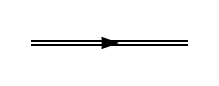
\begin{tikzpicture}[baseline]
				\draw[double,thick] (0,0)-- (2,0);
				\node at (1,0) {\arrow};
			\end{tikzpicture}
			&=
			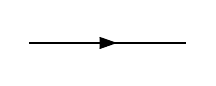
\begin{tikzpicture}[baseline]
				\draw[thick] (0,0)-- (2,0);
				\node at (1,0) {\arrow};
			\end{tikzpicture}
			+
			\left(
			\begin{tikzpicture}
				\draw[thick] (0,0)--(2,0);
				\draw[thick,dashed] (1,1)--(1,0);
				\node at (1,1) {\cross};
			\end{tikzpicture}
			+
			\begin{tikzpicture}
				\draw[thick] (0,0)--(3,0);
				\draw[thick,dashed] (1,1)--(1,0);
				\draw[thick,dashed] (2,1)--(2,0);
				\node at (1,1) {\cross};
				\node at (2,1) {\cross};
			\end{tikzpicture}
			+\cdots\right)\\
			&+
			\left(
			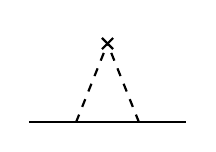
\begin{tikzpicture}
				\draw[thick] (0,0)--(2,0);
				\draw[thick,dashed] (0.6,0)--(1,1);
				\draw[thick,dashed] (1.4,0)--(1,1);
				\node at (1,1) {\cross};
			\end{tikzpicture}
			+
			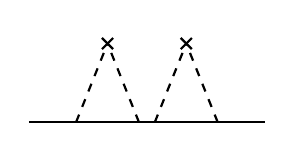
\begin{tikzpicture}
				\draw[thick] (0,0)--(3,0);
				\draw[thick,dashed] (0.6,0)--(1,1);
				\draw[thick,dashed] (1.4,0)--(1,1);
				\draw[thick,dashed] (1.6,0)--(2,1);
				\draw[thick,dashed] (2.4,0)--(2,1);
				\node at (1,1) {\cross};
				\node at (2,1) {\cross};
			\end{tikzpicture}
			+
			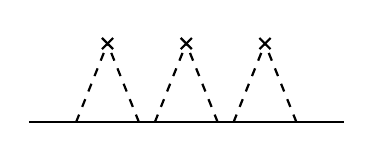
\begin{tikzpicture}
				\draw[thick] (0,0)--(4,0);
				\draw[thick,dashed] (0.6,0)--(1,1);
				\draw[thick,dashed] (1.4,0)--(1,1);
				\draw[thick,dashed] (1.6,0)--(2,1);
				\draw[thick,dashed] (2.4,0)--(2,1);
				\draw[thick,dashed] (2.6,0)--(3,1);
				\draw[thick,dashed] (3.4,0)--(3,1);
				\node at (1,1) {\cross};
				\node at (2,1) {\cross};
				\node at (3,1) {\cross};
			\end{tikzpicture}
			\right)\\
			&+\left(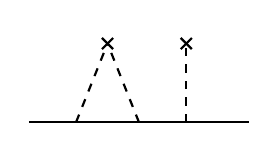
\begin{tikzpicture}
				\draw[thick] (0,0)--(2.8,0);
				\draw[thick,dashed] (0.6,0)--(1,1);
				\draw[thick,dashed] (1.4,0)--(1,1);
				\draw[thick,dashed] (2,0)--(2,1);
				\node at (1,1) {\cross};
				\node at (2,1) {\cross};
			\end{tikzpicture}
			+
			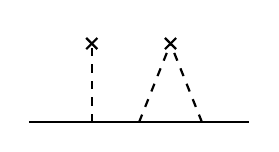
\begin{tikzpicture}
				\draw[thick] (0.2,0)--(3,0);
				\draw[thick,dashed] (1.6,0)--(2,1);
				\draw[thick,dashed] (2.4,0)--(2,1);
				\draw[thick,dashed] (1,0)--(1,1);
				\node at (1,1) {\cross};
				\node at (2,1) {\cross};
			\end{tikzpicture}+\cdots\right)+\cdots,
		\end{align*}
		\iffalse
			\begin{align*}
				\begin{fmfgraph}(80,40)
					\fmfleft{i}
					\fmfright{o}
					\fmf{double_arrow}{i,o}
				\end{fmfgraph}
				&=
				\begin{fmfgraph}(40,40)
					\fmfleft{i}
					\fmfright{o}
					\fmf{fermion}{i,o}
				\end{fmfgraph}
				+
				\left(\begin{fmfgraph}(80,40)
					\fmfleft{i1,i2} \fmfright{o1,o2}
					\fmf{fermion}{i1,d1,o1}
					\fmf{phantom}{i2,u1,o2}
					\fmffreeze
					\fmf{dashes}{d1,u1}
					\fmfv{d.sh=cross}{u1}
				\end{fmfgraph}
				+
				\begin{fmfgraph}(120,40)
					\fmfleft{i1,i2} \fmfright{o1,o2}
					\fmf{fermion}{i1,d1,d2,o1}
					\fmf{phantom}{i2,u1,u2,o2}
					\fmffreeze
					\fmf{dashes}{d1,u1}
					\fmf{dashes}{d2,u2}
					\fmfv{d.sh=cross}{u1}
					\fmfv{d.sh=cross}{u2}
				\end{fmfgraph}
				+
				\begin{fmfgraph}(160,40)
					\fmfleft{i1,i2} \fmfright{o1,o2}
					\fmf{fermion}{i1,d1,d2,d3,o1}
					\fmf{phantom}{i2,u1,u2,u3,o2}
					\fmffreeze
					\fmf{dashes}{d1,u1}
					\fmf{dashes}{d2,u2}
					\fmf{dashes}{d3,u3}
					\fmfv{d.sh=cross}{u1}
					\fmfv{d.sh=cross}{u2}
					\fmfv{d.sh=cross}{u3}
				\end{fmfgraph}
				+\cdots\right)\\
				&+\left(\begin{fmfgraph}(120,40)
					\fmfleft{i1,i2} \fmfright{o1,o2}
					\fmf{fermion}{i1,d1,d2,o1}
					\fmf{phantom}{i2,u1,o2}
					\fmffreeze
					\fmf{dashes}{d1,u1}
					\fmf{dashes}{d2,u1}
					\fmfv{d.sh=cross}{u1}
				\end{fmfgraph}
				+\begin{fmfgraph}(240,40)
					\fmfleft{i1,i2} \fmfright{o1,o2}
					\fmf{fermion}{i1,d1,d2,d3,d4,d5,o1}
					\fmf{phantom}{i2,u1,u2,u3,o2}
					\fmffreeze
					\fmf{dashes}{d1,u1}
					\fmf{dashes}{d2,u1}
					\fmf{dashes}{d4,u3}
					\fmf{dashes}{d5,u3}
					\fmfv{d.sh=cross}{u1}
					\fmfv{d.sh=cross}{u3}
				\end{fmfgraph}
				+\cdots
				\right)+\cdots.
			\end{align*}
		\fi
		which, up to \emph{single-loop} level, can be re-arranged as celebrated Dyson equation
		\begin{equation*}
			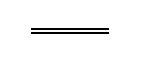
\begin{tikzpicture}
				\draw[double,thick] (0,0)--(1,0);
			\end{tikzpicture}
			=
			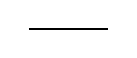
\begin{tikzpicture}
				\draw[thick] (0,0)--(1,0);
			\end{tikzpicture}
			+
			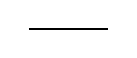
\begin{tikzpicture}
				\draw[thick] (0,0)--(1,0);
			\end{tikzpicture}
			\times
			\left(\begin{tikzpicture}
				\draw[thick,dashed] (0,0)--(0,1);
				\node at (0,1) {\cross};
			\end{tikzpicture}
			+
			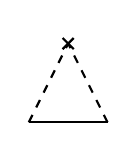
\begin{tikzpicture}
				\draw[thick] (0,0)--(1,0);
				\draw[thick,dashed] (0,0)--(0.5,1);
				\draw[thick,dashed] (1,0)--(0.5,1);
				\node at (0.5,1) {\cross};
			\end{tikzpicture}\right)
			\times
			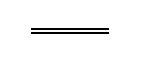
\begin{tikzpicture}
				\draw[double,thick] (0,0)--(1,0);
			\end{tikzpicture},
		\end{equation*}
		or mathematically,
		\begin{equation}\label{2.1.5}
			G_{k,k'}=(G_0)_k+(G_0)_k\Sigma_{k,k''}G_{k',k''},
		\end{equation}
		where the \emph{irreducible self-energy operator}
		\begin{equation*}
			\Sigma_{k,k'}\equiv\langle\bm{k}|T_n|\bm{k'}\rangle\equiv\left(\begin{tikzpicture}
				\draw[thick,dashed] (0,0)--(0,1);
				\node at (0,1) {\cross};
			\end{tikzpicture}
			+
			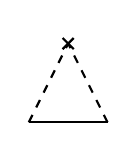
\begin{tikzpicture}
				\draw[thick] (0,0)--(1,0);
				\draw[thick,dashed] (0,0)--(0.5,1);
				\draw[thick,dashed] (1,0)--(0.5,1);
				\node at (0.5,1) {\cross};
			\end{tikzpicture}\right)
		\end{equation*}
		is the single-loop level of T-matrix.\par
		Particularly, since most impurity scattering is momentum-conserving (which is also the case of our s-d Hamiltonian), $\Sigma_{k,k'}=\Sigma_k\delta_{k,k'}$, so Dyson equation \eqref{2.1.5} can be expressed explicitly
		\begin{equation}\label{2.1.6}
			G(i\omega_n,\bm{k})=\dfrac{1}{(G_0)_k^{-1}-\Sigma_k}\equiv\dfrac{1}{i\omega_n-\xi_k-\Sigma_k}.
		\end{equation}
		\indent Besides, with the Dyson equation of retarded and advanced T-matrix (which can be easily seen from equation \eqref{2.1.4})
		\begin{equation*}
			T^{R/A}=\left\langle H_{\imp}\dfrac{1}{\mathds{1}-G_0^{R/A}H_{\imp}}\right\rangle_\imp,
		\end{equation*}
		one immediately has
		\begin{align*}
			T^A(G_0^R-G_0^A)T^R&\equiv H_\imp \dfrac{1}{\mathds{1}-G_0^A H_\imp}\bigg((H_\imp^{-1}-G_0^A)-(H_\imp^{-1}-G_0^R)\bigg)H_\imp \dfrac{1}{\mathds{1}-G_0^R H_\imp}\\
			&=T^R-T^A.
		\end{align*}
		Because
		\begin{equation*}
			\langle\bm{k'}|G_0^R-G_0^A|\bm{k'}\rangle\equiv\dfrac{2i\delta}{(\varepsilon_k- \varepsilon_{k'})^2+\delta^2}=2\pi i\delta(\varepsilon_k- \varepsilon_{k'}).
		\end{equation*}
		\indent \textbf{Analytical properties tell that the imaginary part of the \emph{retarded} self-energy operator (in real time formalism) gives half of the scattering rate}\footnote{For more explanation and discussion, see \cite{altland2010condensed} and \cite{abrikosov2012methods}.}
		\begin{equation*}
		 	\Im\Sigma^R=-\frac{1}{2\tau}.
		 \end{equation*}
		Therefore the relaxation time can be calculated by T-matrix element as following
		\begin{equation}\label{2.1.7}
			\boxed{\dfrac{1}{2\tau}\equiv\Im \Sigma^R(\varepsilon_k,\bm{k})\equiv\Im\langle\bm{k}|T^R|\bm{k}\rangle=\pi\left\langle\sum_{\bm{k'}}|\langle\bm{k'}|T^R|\bm{k}\rangle|^2\delta(\varepsilon_k- \varepsilon_{k'})\right\rangle_{\imp}},
		\end{equation}
		where we utilize the identity $\Re\Sigma^R=\Re \Sigma_A$, $\Im\Sigma^R=-\Im\Sigma^A$ and recover the (single) impurity average.
	
	\subsection{Logarithm Contribution from Spin-flip Process}

\iffalse
	One tempts to utilize \emph{Drude fomula} to connect relaxation time \eqref{2.1.7} we derived before with the conductivity. However, this rude substitution is not correct because forward scattering and backward scattering cannot be symmetric, otherwise electron cannot be transport and the conductance should always be zero.\par
\fi

		Relation of Conductance and relaxation time (of impurity scattering) is given by the famous \emph{Drude formula}\footnote{Strickly speaking, one need to prove by Kubo formula that this semi-classical equation still work for our deliberate consideration of quantum spin impurities. The complete proof is given in \cite{hewson1997kondo}.}
		\begin{equation}\label{2.2.1}
			\sigma=\dfrac{ne^2\tau}{m}.
		\end{equation}
		So to reveal the high-order correction of the temperature dependence of resistence, our left tasks are to evaluate the matrix element of $T$-matrix. More precisely, in our situation, the scattering rate \eqref{2.1.7} is written as
		\begin{equation}\label{2.2.2}
			\Gamma\equiv\dfrac{1}{\tau}=2\pi\left\langle\sum_{\bm{k'},\sigma'}|\langle\bm{k'},\sigma'|T^R|\bm{k},\sigma\rangle|^2\delta(\varepsilon_k- \varepsilon_{k'})\right\rangle_{m_s}
		\end{equation}
		where $\langle\cdots\rangle_{m_s}\equiv\mathrm{tr}_{m_s}(\cdots)/\mathrm{tr}_{m_s}(\mathds{1})=\mathrm{tr}_{m_s}(\cdots)/(2S+1)\hbar^2$ and $T^R$ is given perturbatively from \eqref{2.1.4}. Scattering processes become much more clear if the Hamiltonian is split to \emph{non-spin-flip} part ($S_d^z$) and \emph{spin-flip} parts ($S_d^\pm$)
		\begin{equation}\label{2.2.3}
			H_\imp=J\sum_{kk'}\bm{S}_{k,k'}\cdot\bm{S}_d\equiv J\sum_{k_1,k_2}\bigg[\left(a_{k1\uparrow}^\dagger a_{k_2\uparrow}-a_{k_1\downarrow}^\dagger a_{k_2\downarrow}\right)S_d^z+a_{k_1\downarrow}^\dagger a_{k_2\uparrow}S_d^+ +a_{k_1\uparrow}^\dagger a_{k_2\downarrow}S_d^-\bigg].
		\end{equation}
		So to the lowest order of $T$-matrix where $T^R=H_\imp$, only spin flipping and non-flipping processes will be involved
		\begin{align}
			\dfrac{1}{2\tau}&=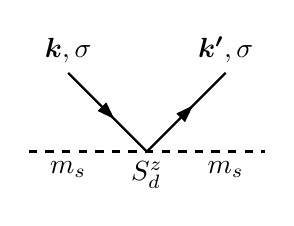
\begin{tikzpicture}[baseline]
				\draw[thick,dashed] (-1.5,0)--(1.5,0);
				\draw[thick] (-1,1)--(0,0)--(1,1);
				\node[below] at (1,0) {$m_s$};
				\node[below] at (-1,0) {$m_s$};
				\node[below] at (0,0) {$S_d^z$};
				\node[rotate=-45] at (-0.5,0.5) {\arrow};
				\node[above] at (-1,1) {$\bm{k},\sigma$};
				\node[above] at (1,1) {$\bm{k'},\sigma$};
				\node[rotate=45] at (0.5,0.5) {\arrow};
			\end{tikzpicture}+
			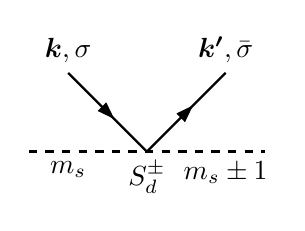
\begin{tikzpicture}[baseline]
				\draw[thick,dashed] (-1.5,0)--(1.5,0);
				\draw[thick] (-1,1)--(0,0)--(1,1);
				\node[below] at (1,0) {$m_s\pm1$};
				\node[below] at (-1,0) {$m_s$};
				\node[below] at (0,0) {$S_d^\pm$};
				\node[rotate=-45] at (-0.5,0.5) {\arrow};
				\node[above] at (-1,1) {$\bm{k},\sigma$};
				\node[above] at (1,1) {$\bm{k'},\bar{\sigma}$};
				\node[rotate=45] at (0.5,0.5) {\arrow};
			\end{tikzpicture}\nonumber\\
			&=\dfrac{\pi J^2}{(2S+1)\hbar^2}\sum_{m_s}\sum_{\bm{k'}}\left[2|\langle m_s|S_d^z|m_s\rangle|^2+\bigg(|\langle m_s-1|S_d^+|m_s\rangle|^2+|\langle m_s+1|S_d^-|m_s\rangle|^2\bigg)\right]\delta(\varepsilon_{\bm{k}}-\varepsilon_{\bm{k'}})\nonumber\\
			&=\dfrac{\pi J^2 n}{(2S+1)\hbar^2}\sum_{m_s}\bigg[2\hbar^2m_s^2+\hbar^2\big(S(S+1)-(m-1)m\big)+\hbar^2\big(S(S+1)-(m+1)m\big)\bigg]\nonumber\\
			&=\dfrac{\pi J^2 n}{2S+1}\sum_{m_s}\left(S(S+1)+2m_s\right)=\pi J^2 nS(S+1),\label{2.2.4}
		\end{align}
		where $2$ in the first line comes from wick contraction of itinerate fermionic operators, and the DOS $n$ is a constant (for our itinerate electrons $|\bm{k}|\simeq k_F$).\par
		Clearly \eqref{2.2.4} has no temperature dependence so it cannot contribute to the behavior of resistance minimum. In fact, one can easily see that the only possible involvement of temperature comes from the fermionic distrbution of intermediate states. So only if we take the free Green function into account, i.e., start with the second order of the perturbative series of $T^R$, can we have the desired temperature dependence.\par
		But things becomes dramatically complex when we go to the second order. As is seen below, there will be six diagrams (including in and out spin degenerancy) contributing to relaxation time\footnote{One can easily check that terms like $\langle|\hat{S_d^z}\hat{G}_0\hat{S}_d^\pm|\rangle$ vanish because single creation or annihilation operator will survive after contraction, whose expectation value is always zero.}
		\begin{align}
			&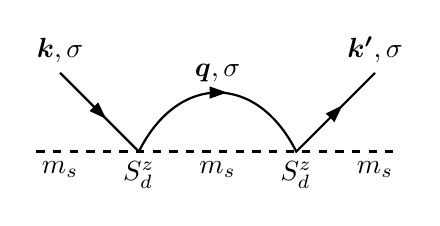
\begin{tikzpicture}[baseline]
				\draw[thick,dashed] (-2.3,0)--(2.3,0);
				\draw[thick] (-2,1)--(-1,0) .. controls (-0.5,1) and (0.5,1) ..(1,0)--(2,1);
				\node[below] at (2,0) {$m_s$};
				\node[below] at (-2,0) {$m_s$};
				\node[below] at (0,0) {$m_s$};
				\node[below] at (1,0) {$S_d^z$};
				\node[below] at (-1,0) {$S_d^z$};
				\node[rotate=-45] at (-1.5,0.5) {\arrow};
				\node at (0,0.75) {\arrow};
				\node at (0,1) {$\bm{q},\sigma$};
				\node[above] at (-2,1) {$\bm{k},\sigma$};
				\node[above] at (2,1) {$\bm{k'},\sigma$};
				\node[rotate=45] at (1.5,0.5) {\arrow};
			\end{tikzpicture}+
			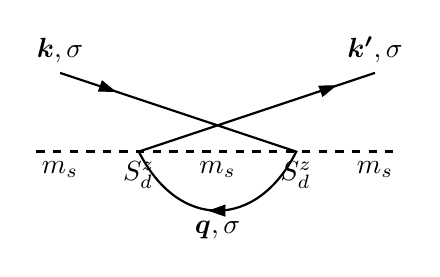
\begin{tikzpicture}[baseline]
				\draw[thick,dashed] (-2.3,0)--(2.3,0);
				\draw[thick] (-2,1)--(1,0) .. controls (0.5,-1) and (-0.5,-1) .. (-1,0)--(2,1);
				\node[below] at (2,0) {$m_s$};
				\node[below] at (-2,0) {$m_s$};
				\node[below] at (0,0) {$m_s$};
				\node[below] at (1,0) {$S_d^z$};
				\node[below] at (-1,0) {$S_d^z$};
				\node[rotate=-20] at (-1.4,0.8) {\arrow};
				\node[rotate=180] at (0,-0.75) {\arrow};
				\node at (0,-1) {$\bm{q},\sigma$};
				\node[above] at (-2,1) {$\bm{k},\sigma$};
				\node[above] at (2,1) {$\bm{k'},\sigma$};
				\node[rotate=20] at (1.4,0.8) {\arrow};
			\end{tikzpicture}+
			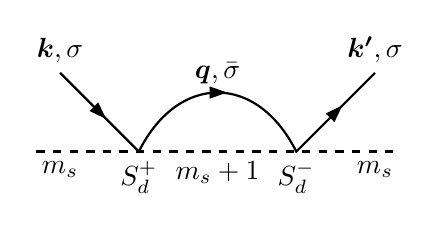
\begin{tikzpicture}[baseline]
				\draw[thick,dashed] (-2.3,0)--(2.3,0);
				\draw[thick] (-2,1)--(-1,0) .. controls (-0.5,1) and (0.5,1) ..(1,0)--(2,1);
				\node[below] at (-2,0) {$m_s$};
				\node[below] at (0,0) {$m_s+1$};
				\node[below] at (2,0) {$m_s$};
				\node[below] at (1,0) {$S_d^-$};
				\node[below] at (-1,0) {$S_d^+$};
				\node[rotate=-45] at (-1.5,0.5) {\arrow};
				\node at (0,0.75) {\arrow};
				\node at (0,1) {$\bm{q},\bar{\sigma}$};
				\node[above] at (-2,1) {$\bm{k},\sigma$};
				\node[above] at (2,1) {$\bm{k'},\sigma$};
				\node[rotate=45] at (1.5,0.5) {\arrow};
			\end{tikzpicture}\nonumber\\
			&+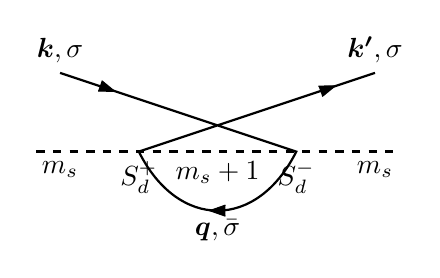
\begin{tikzpicture}[baseline]
				\draw[thick,dashed] (-2.3,0)--(2.3,0);
				\draw[thick] (-2,1)--(1,0) .. controls (0.5,-1) and (-0.5,-1) .. (-1,0)--(2,1);
				\node[below] at (-2,0) {$m_s$};
				\node[below] at (0,0) {$m_s+1$};
				\node[below] at (2,0) {$m_s$};
				\node[below] at (1,0) {$S_d^-$};
				\node[below] at (-1,0) {$S_d^+$};
				\node[rotate=-20] at (-1.4,0.8) {\arrow};
				\node[rotate=180] at (0,-0.75) {\arrow};
				\node at (0,-1) {$\bm{q},\bar\sigma$};
				\node[above] at (-2,1) {$\bm{k},\sigma$};
				\node[above] at (2,1) {$\bm{k'},\sigma$};
				\node[rotate=20] at (1.4,0.8) {\arrow};
			\end{tikzpicture}+
			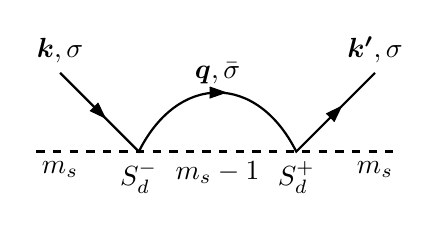
\begin{tikzpicture}[baseline]
				\draw[thick,dashed] (-2.3,0)--(2.3,0);
				\draw[thick] (-2,1)--(-1,0) .. controls (-0.5,1) and (0.5,1) ..(1,0)--(2,1);
				\node[below] at (-2,0) {$m_s$};
				\node[below] at (0,0) {$m_s-1$};
				\node[below] at (2,0) {$m_s$};
				\node[below] at (1,0) {$S_d^+$};
				\node[below] at (-1,0) {$S_d^-$};
				\node[rotate=-45] at (-1.5,0.5) {\arrow};
				\node at (0,0.75) {\arrow};
				\node at (0,1) {$\bm{q},\bar{\sigma}$};
				\node[above] at (-2,1) {$\bm{k},\sigma$};
				\node[above] at (2,1) {$\bm{k'},\sigma$};
				\node[rotate=45] at (1.5,0.5) {\arrow};
			\end{tikzpicture}+
			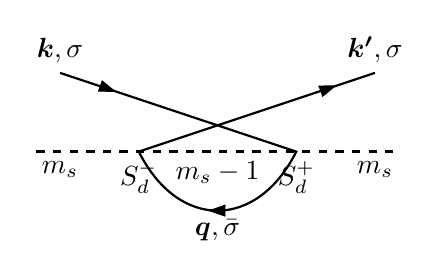
\begin{tikzpicture}[baseline]
				\draw[thick,dashed] (-2.3,0)--(2.3,0);
				\draw[thick] (-2,1)--(1,0) .. controls (0.5,-1) and (-0.5,-1) .. (-1,0)--(2,1);
				\node[below] at (-2,0) {$m_s$};
				\node[below] at (0,0) {$m_s-1$};
				\node[below] at (2,0) {$m_s$};
				\node[below] at (1,0) {$S_d^+$};
				\node[below] at (-1,0) {$S_d^-$};
				\node[rotate=-20] at (-1.4,0.8) {\arrow};
				\node[rotate=180] at (0,-0.75) {\arrow};
				\node at (0,-1) {$\bm{q},\bar\sigma$};
				\node[above] at (-2,1) {$\bm{k},\sigma$};
				\node[above] at (2,1) {$\bm{k'},\sigma$};
				\node[rotate=20] at (1.4,0.8) {\arrow};
			\end{tikzpicture}.\label{2.2.5}
		\end{align}
\iffalse
		Without calculating scattering amplitudes in \eqref{2.2.5} term by term, where the discussion is extremely tedious, here we try to work them out together. First note that state $H_\imp|\bm{k'},\sigma'\rangle$ consists of a single-particle state and a two-particle-one-hole state
		\begin{align}\label{2.2.6}
			H_\imp|\bm{k'},\sigma'\rangle&=J\sum_{p_1\mu_1p_2\mu_2}c_{p_1\mu_2}^\dagger\dfrac{\bm{\sigma}_{\mu_1\mu_2}\cdot\bm{S}_d}{2}c_{p_2\mu_2}c_{k'\sigma'}^\dagger|\Omega\rangle\nonumber\\
			&=J\sum_{p_1\mu_1}\dfrac{\bm{\sigma}_{\mu_1\sigma'}\cdot\bm{S}_d}{2}c_{p_1\mu_1}^\dagger|\Omega\rangle-J\sum_{p_1\mu_1p_2\mu_2}\dfrac{\bm{\sigma}_{\mu_1\mu_2}\cdot\bm{S}_d}{2}c_{p_1\mu_2}^\dagger c_{k'\sigma'}^\dagger c_{p_2\mu_2}|\Omega\rangle,
		\end{align}
		whose energies are $\varepsilon_{p_1}$ and $\varepsilon_{p_1}+\varepsilon_{k'}-\varepsilon_{p_2}$, respectively. So mutiplying bra state $\langle\bm{k},\sigma|H_\imp$ and observing that only the overlap of single-particle-single-particle pair and two-particle-one-hole-two-particle-one-hole pair will be non-vanishing, we have
		\begin{align}
			\langle\bm{k},\sigma|T^{(2)}|\bm{k'},\sigma'\rangle&=\dfrac{J^2}{4}(\sigma_{\sigma\mu_1'}\cdot\bm{S}_d)(\sigma_{\mu_1\sigma}\cdot\bm{S}_d)\sum_{p_1p_1'}\dfrac{\langle\Omega|c_{p_1'\mu_1'}c_{p_1\mu_1}^\dagger|\Omega\rangle}{\varepsilon_k- \varepsilon_{p_1}+i\delta}+\nonumber\\
			&=\dfrac{J^2}{4}(\sigma_{\mu_2'\mu_1'}\cdot\bm{S}_d)(\sigma_{\mu_1\mu_2}\cdot\bm{S}_d)\sum_{p_1p_2p_1'p_2'}\dfrac{\langle\Omega|{\color{red}c_{p_2'\mu_2'}^\dagger c_{k\sigma} c_{p_1'\mu_1'}}{\color{blue}c_{p_1\mu_1}^\dagger c_{k'\sigma'}^\dagger c_{p_2\mu_2}}|\Omega\rangle}{\varepsilon_k- \varepsilon_{p_1}-\varepsilon_{k'}+\varepsilon_{p_2}},\label{2.2.7}
		\end{align}
		where in the second line I emphasize the state consisting of two-particle and one-hole.\par
		All the disconnected ``vacuum'' bubble diagrams (here ``vacuum'' is the Fermi sphere) in the second term of \eqref{2.2.7}, i.e., those that contains contraction in the same state (either red-red or blue-blue contraction) will be absorbed in the normalization of partition function. So the only non-trivial term comes from the contraction $\langle\Omega|{\color{red}c_{p_2'\mu_2'}^\dagger\color{blue}c_{p_2\mu_2}}|\Omega\rangle\langle\Omega|{\color{red}c_{k\sigma} c_{p_1'\mu_1'}}{\color{blue}c_{p_1\mu_1}^\dagger c_{k'\sigma'}^\dagger }$
\fi
		Although there are up to six feynman diagrams waiting to be calculated, there contraction rules are similar to each other. Let us taking one typical process of from state $|\bm{k},\uparrow\rangle$ to $|\bm{k'},\uparrow\rangle$ as an example% (impurities are made of electron so $S_d=1/2$ in our situation).
		\begin{align*}
			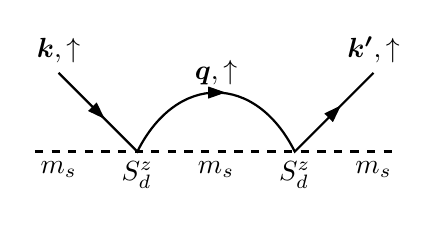
\begin{tikzpicture}[baseline]
				\draw[thick,dashed] (-2.3,0)--(2.3,0);
				\draw[thick] (-2,1)--(-1,0) .. controls (-0.5,1) and (0.5,1) ..(1,0)--(2,1);
				\node[below] at (2,0) {$m_s$};
				\node[below] at (-2,0) {$m_s$};
				\node[below] at (0,0) {$m_s$};
				\node[below] at (1,0) {$S_d^z$};
				\node[below] at (-1,0) {$S_d^z$};
				\node[rotate=-45] at (-1.5,0.5) {\arrow};
				\node at (0,0.75) {\arrow};
				\node at (0,1) {$\bm{q},\uparrow$};
				\node[above] at (-2,1) {$\bm{k},\uparrow$};
				\node[above] at (2,1) {$\bm{k'},\uparrow$};
				\node[rotate=45] at (1.5,0.5) {\arrow};
			\end{tikzpicture}+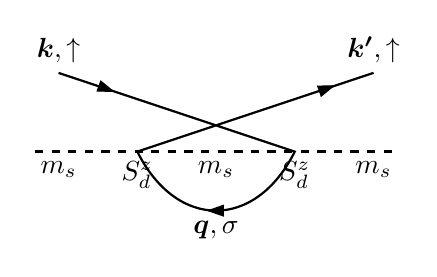
\begin{tikzpicture}[baseline]
				\draw[thick,dashed] (-2.3,0)--(2.3,0);
				\draw[thick] (-2,1)--(1,0) .. controls (0.5,-1) and (-0.5,-1) .. (-1,0)--(2,1);
				\node[below] at (2,0) {$m_s$};
				\node[below] at (-2,0) {$m_s$};
				\node[below] at (0,0) {$m_s$};
				\node[below] at (1,0) {$S_d^z$};
				\node[below] at (-1,0) {$S_d^z$};
				\node[rotate=-20] at (-1.4,0.8) {\arrow};
				\node[rotate=180] at (0,-0.75) {\arrow};
				\node at (0,-1) {$\bm{q},\sigma$};
				\node[above] at (-2,1) {$\bm{k},\uparrow$};
				\node[above] at (2,1) {$\bm{k'},\uparrow$};
				\node[rotate=20] at (1.4,0.8) {\arrow};
			\end{tikzpicture}\\= J^2\left\langle\Omega\left|{\color{magenta}c_{k\uparrow}}\sum_{p_1p_2p_3p_4}{\color{red}\left(c_{p_1\uparrow}^\dagger c_{p_2\uparrow}-c_{p_1\downarrow}^\dagger c_{p_2\downarrow}\right)}S_d^z \hat{G}_0{\color{blue}\left(c_{p_3\uparrow}^\dagger c_{p_4\uparrow}-c_{p_3\downarrow}^\dagger c_{p_4\downarrow}\right)}S_d^z{\color{magenta}c_{k'\uparrow}^\dagger}\right|\Omega\right\rangle,
		\end{align*}
		where different colors are utilized to emphase the physical operators that creation and annihilation operators belongs to. \textbf{Since we are considering \emph{irreducible self-energy operators}, all the factorized feynman digrams (bubble diagrams) coming from contraction within the same physical operators should be excluded from our calculation. These vacuum contribution will be absorbed in the normalization of path integral}. Also, $T$-matrix only focus on the contribution that $|\bm{k},\sigma\rangle\neq|\bm{k'}\sigma'\rangle$ (the trivial divergent part of $|\bm{k},\sigma\rangle=|\bm{k'},\sigma'\rangle$ is included in definition of $S$-matrix, rather than our $T$-matrix\footnote{If you are not familiar with this, see \cite{weinberg1995quantum} for more details.}) so we use the same color to avoid contraction between them. And free Green function $\hat{G}_0\equiv1/(\varepsilon_k-\hat{H}+i\delta)$ depends on the state after arrange of the order of operators for contraction. Therefore, the only non-vanishing contraction is
		\begin{align}
			J^2\sum_{p_1p_2p_3p_4}\langle\Omega|{\color{magenta}c_{k\uparrow}}{\color{red}c_{p_1\uparrow}^\dagger c_{p_2\uparrow}}S_d^z \hat{G}{\color{blue}c_{p_3\uparrow}^\dagger c_{p_4\uparrow}}S_d^z{\color{magenta}c_{k'\uparrow}^\dagger}|\Omega\rangle&=J^2\sum_{p_1p_2p_3p_4}\langle c_{k\uparrow} c_{p_1\uparrow}^\dagger\rangle S_d^z\dfrac{\langle c_{p_2\uparrow} c_{p_3\uparrow}^\dagger\rangle}{\varepsilon_k- \varepsilon_{p_2}+i\delta}S_d^z\langle c_{p_4\uparrow} c_{k'\uparrow}^\dagger\rangle\nonumber\\
			&+J^2\sum_{p_1p_2p_3p_4}\langle c_{k\uparrow} c_{p_3\uparrow}^\dagger\rangle S_d^z\dfrac{\langle c_{p_1\uparrow}^\dagger c_{p_4\uparrow}\rangle}{\varepsilon_k-\varepsilon_{p_4}+i\delta}S_d^z\langle c_{p_2\uparrow} c_{k'\uparrow}^\dagger\rangle\nonumber\\
			&=J^2\sum_p\dfrac{1-f(\varepsilon_p)}{\varepsilon_k- \varepsilon_p+i\delta}S_d^z+J^2\sum_p\dfrac{f(\varepsilon_p)}{\varepsilon_k- \varepsilon_p+i\delta}S_d^z,\label{2.2.6}
		\end{align}
		which is not temperature-dependent again. By replacing $S_d^z$ by $S^\pm$, and dropping all the temperature-independent terms, we arrive at the final simple expression
		\begin{align}
			\langle\bm{k},\sigma|T^{R(2)}|\bm{k'},\sigma\rangle&\xlongequal{\text{temp.-depend}}-J^2\sum_p[S^+,S^-]\dfrac{f(\varepsilon_p)}{\varepsilon_k- \varepsilon_p+i\delta}=-J^2\sum_p\dfrac{f(\varepsilon_p)}{\varepsilon_k- \varepsilon_p+i\delta}2S_d^z\nonumber\\
			&=-2J^2S^z\left(n\mathcal{P.V.}\int_{-D}^D\,\dd \varepsilon_p\dfrac{f(\varepsilon_p)}{\varepsilon_k- \varepsilon_p+i\delta}-i\pi n\right)=2J^2nS_d^z\ln\left|\dfrac{D}{k_BT}\right|\label{2.2.7}
		\end{align}
		for $\varepsilon_k\ll D$ and $\varepsilon_k- \varepsilon_F\simeq k_BT$. Therefore, after plugging in \eqref{2.1.7}, performing the integral over $\bm{k'}$ and taking the trace of impurity spins, we arrive at the final single-loop correction on the relaxation time
		\begin{equation}\label{2.2.8}
			\dfrac{1}{2\tau}=\pi n J^2S(S+1)\left(1+2nJ\ln\left|\dfrac{D}{k_BT}\right|\right)^2\simeq\pi n J^2S(S+1)\left(1+4nJ\ln\left|\dfrac{D}{k_BT}\right|+\cdots\right).
		\end{equation}
		And thus the resistance will contain a temperature-dependent and logarithmically divergent term $\ln|D/k_BT|$ as well (plus the phonon-contribution\footnote{This can be derived from Boltzman equation by taking into account all the eletron-phonon scattering processes. See chapter 11 of \cite{phillips2012advanced} for details.} that is proportional to $T^5$)
		\begin{equation}\label{2.2.9}
			R(T)\sim AT^5+R(0)\left(1-4n J\ln\left|\dfrac{k_BT}{D}\right|+\cdots\right).
		\end{equation}
		This logarithmical correction will bend up the curve when decreasing the temperature for \emph{antiferromagnetic coupling} (but not ferromagnetic coupling) so can well-explain the existence of resistence minimum for alloys \cite{kondo1964resistance}.

\section{Kondo Problem}
	\subsection{Poor Man's Scaling: Renormalization}
		One may be satisfied with our logarithmical correction \eqref{2.2.9} that matches well with experiments. However, this is still not the end. If we continue decreasing the temperature, equation \eqref{2.2.9} tells us that the resistance of alloy will goes to infinity at zero temperature, which is thoroughly unacceptable.\par
		But to explain the minimum of resistance, we do need this logarithmical-divergent term. So here comes the contradiction: \textbf{the logarithmical-divergent term works well in low energy (small $T$) region, but become untrusted when we go further to lower energy scale.} But to those having deep insights of condensed matter physics like Anderson, contradiction can also be understood as some hints of deep physics behind. Actually, it tells us that {\color{red}\textbf{there will be one critial temperature or critical energy scale under which our perturbative treatment of scattering processes break down}}. And because perturbation theory is built on the assumption of small coupling constant, the only conclusion we can draw is that {\color{red}\textbf{the coupling constant must run with the scaling factor until divergence when we lower the temperature}}. This is nothing but the concept of \textbf{renormalization group flow}.
		
	\subsection{Schrieffer-Wolff Transformation Again}
		In order to visualize the low-energy behavior of coupling constants, we need to scaling the conduction band into two parts $(-D/b,D/b)$ and $(-D,-D/b]\cup[D/b,D)$ for $b>1$ and decomposing the many-body Hilbert spcae into three kinds\footnote{Because doubly excited intermediate states are of high order} with the same notation (but different meaning) in the first section: $\psi_1$ has no conduction electron or hole in the upper and lower edge, $\psi_0$ has at least one hole in the lower edge, and $\psi_2$ has at least one conduction electron in the upper edge.\par
		For further discussion Anderson consider a generalized \emph{anisotropic} s-d Hamiltonian in his original work in \cite{anderson1970poor}
		\begin{equation}\label{3.1.1}
			H_{\text{sd}}=\sum_{kk'}\bigg(J_zS^z(c_{k\uparrow}^\dagger c_{k'\uparrow}-c_{k\downarrow}^\dagger c_{k'\downarrow})+J_+S^+c_{k\downarrow}^\dagger c_{k'\uparrow}+J_-S^-c_{k\uparrow}^\dagger c_{k'\downarrow}\bigg).
		\end{equation}
		Scaling of the momentum space will result in the seperation of summation
		\begin{equation*}
			\sum_k\equiv\sum_{|k|\in(0,D/b)}+\sum_{|k|\in(D/b,D)}\equiv\sum_{k_\ell}+\sum_{k_h}.
		\end{equation*}
		So \eqref{3.1.1} is splitted as
		\begin{align*}
			H_{\text{sd-}\ell\ell}&=\sum_{k_\ell k_\ell'}\bigg(J_zS^z(c_{k_\ell\uparrow}^\dagger c_{k_\ell'\uparrow}-c_{k_\ell\downarrow}^\dagger c_{k_\ell'\downarrow})+J_+S^+c_{k_\ell\downarrow}^\dagger c_{k_\ell'\uparrow}+J_-S^-c_{k_\ell\uparrow}^\dagger c_{k_\ell'\downarrow}\bigg),\\
			H_{\text{sd-}\ell h}&=\sum_{k_\ell k_h'}\bigg(J_zS^z(c_{k_\ell\uparrow}^\dagger c_{k_h'\uparrow}-c_{k_\ell\downarrow}^\dagger c_{k_h'\downarrow})+J_+S^+c_{k_\ell\downarrow}^\dagger c_{k_h'\uparrow}+J_-S^-c_{k_\ell\uparrow}^\dagger c_{k_h'\downarrow}\bigg),\\
			H_{\text{sd-}h \ell}&=\sum_{k_h k_\ell'}\bigg(J_zS^z(c_{k_h\uparrow}^\dagger c_{k_\ell'\uparrow}-c_{k_h\downarrow}^\dagger c_{k_\ell'\downarrow})+J_+S^+c_{k_h\downarrow}^\dagger c_{k_\ell'\uparrow}+J_-S^-c_{k_h\uparrow}^\dagger c_{k_\ell'\downarrow}\bigg),\\
			H_{\text{sd-}h h}&=\sum_{k_h k_h'}\bigg(J_zS^z(c_{k_h\uparrow}^\dagger c_{k_h'\uparrow}-c_{k_h\downarrow}^\dagger c_{k_h'\downarrow})+J_+S^+c_{k_h\downarrow}^\dagger c_{k_h'\uparrow}+J_-S^-c_{k_h\uparrow}^\dagger c_{k_h'\downarrow}\bigg).
		\end{align*}
		Since Hamiltonian \eqref{3.1.1} relates only $\psi_0$ and $\psi_1$ subspace and $\psi_2$ and $\psi_1$ subspace, the effective Hamiltonian should be entirely the same as \eqref{1.2.9} after Schrieffer-Wolff transformation, where
		\begin{equation*}
			H_{11}=H_0+H_{\text{sd-}\ell\ell},\quad H_{00}=H_0+H_{\text{sd-}hh}\text{ for }k_h\in(-D,-D/b),\quad H_{22}=H_0+H_{\text{sd-}hh}\text{ for }k_h\in(D/b,D)
		\end{equation*}
		and
		\begin{align*}
			H_{01}&=H_{\text{sd-}h\ell}\text{ for }k_h\in(-D,-D/b), &H_{10}&=H_{\text{sd-}\ell h}\text{ for }k_h\in(-D,-D/b)\\
			H_{21}&=H_{\text{sd-}h\ell}\text{ for }k_h\in(D/b,D), &H_{12}&=H_{\text{sd-}\ell h}\text{ for }k_h\in(D/b,D).
		\end{align*}
		Here $H_0$ is the kinetic term of free itinerate electrons $H_0=\sum_{k_\ell}\varepsilon_{k_\ell} c_{k_\ell}^\dagger c_{k_\ell}$. To the lowest order of Green function, we can safely approximate
		\begin{equation*}
			H_{11}=H_{00}=H_{22}=H_0+\mathcal{O}(J).
		\end{equation*}
	\subsection{Single-loop $\beta$-function and Asymptotic Freedom}
		We will show in this section that \textbf{the effective Hamiltonian has exactly the same form of the second-order spin scattering processes} (just a coincidence).\par
		Let us first focus on the spin scattering process that keep the spin of impurity unchanged, i.e., the two spin-flip and non spin-flip processes.
		\begin{align}
		 	H_{12}\dfrac{1}{E-H_{22}}H_{21}&=J_zJ_z\sum_{k_{\ell1} k_{h1}'}S^z(c_{k_{\ell1}\uparrow}^\dagger c_{k_{h1}'\uparrow}-c_{k_{\ell1}\downarrow}^\dagger c_{k_{h1}'\downarrow})\dfrac{1}{E-H_{22}}\sum_{k_{h2}'k_{\ell2} }S^z(c_{k_{h2}'\uparrow}^\dagger c_{k_{\ell2}\uparrow}-c_{k_{h2}\downarrow}^\dagger c_{k_{\ell2}'\downarrow})\nonumber\\
		 	&+J_-J_+\sum_{k_{\ell1}k_{h1}'} S^-a_{k_{\ell1}\uparrow}^\dagger a_{k_{h1}'\downarrow}\dfrac{1}{E-H_{22}}\sum_{k_{h2}'k_{\ell2}}S^+ a_{k_{h2}'\downarrow}^\dagger a_{k_{\ell2}\uparrow}\nonumber\\
		 	&+J_+J_-\sum_{k_{\ell1}k_{h1}'} S^+a_{k_{\ell1}\downarrow}^\dagger a_{k_{h1}'\uparrow}\dfrac{1}{E-H_{22}}\sum_{k_{h2}'k_{\ell2}}S^- a_{k_{h2}'\uparrow}^\dagger a_{k_{\ell2}\downarrow}.\label{3.1.2}
		\end{align}
		Moving the creation and annihilation pair on the right hand side to the left hand side of free Green function. Then with the same trick we proved before\footnote{Let me remind you about what I have proved in the first section. If $[H_0,A]=\lambda A$, then \begin{equation*}
			\dfrac{1}{E-H_0}A=A\dfrac{1}{E-\lambda-H_0}.
		\end{equation*}}, because
		\begin{equation*}
			[H_0,a_{k_{h2}'\mu}^\dagger a_{k_{\ell2}\nu}]=a_{k_{h2}'\mu}^\dagger a_{k_{\ell2}\nu}(\varepsilon_{k_{h2}'}-\varepsilon_{k_{\ell2}})\simeq a_{k_{h2}'\mu}^\dagger a_{k_{\ell2}\nu}(D-\varepsilon_{k_{\ell2}})
		\end{equation*}
		and in $\psi_1$ subspace the band edge is empty\footnote{Even without writting the projection explicitly, one must be clear about this.} so that $a_{k_{h1}'\mu_1}a_{k_{h2}'\mu_2}^\dagger=\delta_{k_{h1}',k_{h2}'}\delta_{\mu_1,\mu_2}$ after projection, we are left with
		\begin{align}
			H_{12}\dfrac{1}{E-H_{22}}H_{21}&=J_z^2(S^z)^2\sum_{k_{\ell1}k_{\ell2}}\sum_{k_h}c_{k_{\ell1}\uparrow}^\dagger c_{k_h\uparrow}\dfrac{1}{E-D+\varepsilon_{k_{\ell2}}} c_{k_h\uparrow}^\dagger c_{k_{\ell2}\uparrow}+J_z^2(S^z)^2\sum_{k_{\ell1}k_{\ell2}}\sum_{k_h}c_{k_{\ell1}\downarrow}^\dagger c_{k_h\downarrow}\dfrac{1}{E-D+\varepsilon_{k_{\ell2}}} c_{k_h\downarrow}^\dagger c_{k_{\ell2}\downarrow}\nonumber\\
			&+J_-J_+\left(S^-S^+\sum_{k_{\ell1}k_{\ell2}}\sum_{k_h}c_{k_{\ell1}\uparrow}^\dagger c_{k_h\downarrow}\dfrac{1}{E-D+\varepsilon_{k_{\ell2}}} c_{k_h\downarrow}^\dagger c_{k_{\ell2}\uparrow}+S^+ S^-\sum_{k_{\ell1}k_{\ell2}}\sum_{k_h}c_{k_{\ell1}\downarrow}^\dagger c_{k_h\uparrow}\dfrac{1}{E-D+\varepsilon_{k_{\ell2}}} c_{k_h\uparrow}^\dagger c_{k_{\ell2}\downarrow}\right)\nonumber\\
			&=\dfrac{3J_z^2}{4}\sum_{k_{\ell1}k_{\ell2}}\sum_\sigma \dfrac{c_{k_{\ell1}\sigma}^\dagger c_{k_{\ell2}\sigma}}{E-D+\varepsilon_{k_{\ell2}}}\times n_0D\left(1-\dfrac{1}{b}\right)\nonumber\\
			&+J_-J_+\left\{\left(\dfrac{1}{2}-S^z\right)\sum_{k_{\ell1}k_{\ell2}}\dfrac{c_{k_{\ell1}\uparrow}^\dagger  c_{k_{\ell2}\uparrow}}{E-D+\varepsilon_{k_{\ell2}}}+\left(\dfrac{1}{2}+S^z\right)\sum_{k_{\ell1}k_{\ell2}}\dfrac{c_{k_{\ell1}\downarrow}^\dagger c_{k_{\ell2}\downarrow}}{E-D+\varepsilon_{k_{\ell2}}}\right\}\times n_0D\left(1-\dfrac{1}{b}\right)\label{3.1.3}
		\end{align}
		because $S_z^2=\dfrac{3}{4}$, $S^-S^+=\dfrac{1}{2}-S^z$ and
		\begin{equation*}
			\sum_{k_h}1\equiv\int_{D/b}^{D}\dd\varepsilon\,n(\varepsilon)=n_0D\left(1-\dfrac{1}{b}\right),
		\end{equation*}
		where we approximate the DOS as a constant function within our band as we have done in Kondo effects. Similarly, for another term
		\begin{align}
			H_{10}\dfrac{1}{E-H_{00}}H_{01}&=\dfrac{3J_z^2}{4}\sum_{k_{\ell1}k_{\ell2}}\sum_\sigma\dfrac{c_{k_{\ell1}\sigma}^\dagger c_{k_{\ell2}\sigma}}{E-D-\varepsilon_{k_{\ell2}}}\times n_0D\left(1-\dfrac{1}{b}\right)\nonumber\\
			&+J_-J_+\left\{\left(\dfrac{1}{2}-S^z\right)\sum_{k_{\ell1}k_{\ell2}}\dfrac{c_{k_{\ell1}\uparrow}^\dagger  c_{k_{\ell2}\uparrow}}{E-D-\varepsilon_{k_{\ell2}}}+\left(\dfrac{1}{2}+S^z\right)\sum_{k_{\ell1}k_{\ell2}}\dfrac{c_{k_{\ell1}\downarrow}^\dagger c_{k_{\ell2}\downarrow}}{E-D-\varepsilon_{k_{\ell2}}}\right\}\times n_0D\left(1-\dfrac{1}{b}\right).\label{3.1.4}
		\end{align}
		\indent Ditto for the the other single spin-flip processes that contribute to effective Hamiltonian, which gives
		\begin{align}
			H_{12}\dfrac{1}{E-H_{22}}H_{21}&=-\dfrac{J_z J_+}{2}\sum_{k_{\ell1}k_{\ell2}}\sum_\sigma\dfrac{c_{k_{\ell1}\sigma}^\dagger c_{k_{\ell2}\sigma}}{E-D-\varepsilon_{k_{\ell2}}}\times n_0D\left(1-\dfrac{1}{b}\right),\label{3.1.5}\\
			H_{10}\dfrac{1}{E-H_{00}}H_{01}&=-\dfrac{3J_z J_-}{2}\sum_{k_{\ell1}k_{\ell2}}\sum_\sigma\dfrac{c_{k_{\ell1}\sigma}^\dagger c_{k_{\ell2}\sigma}}{E-D-\varepsilon_{k_{\ell2}}}\times n_0D\left(1-\dfrac{1}{b}\right).\label{3.1.6}
		\end{align}
		Dropping all the trivial shift on effective Hamiltonian (which can be absorbed in the measure of path integral) and recognizing the corresponding terms, finally we obtain
		\begin{align}
			J_\pm(b)&=J_\pm+J_zJ_\pm nD\left(1-\dfrac{1}{b}\right)\left(\dfrac{1}{E-D+\varepsilon_k}+\dfrac{1}{E-D- \varepsilon_k}\right),\label{3.1.7}\\
			J_z(b)&=J_z+J_+J_- nD\left(1-\dfrac{1}{b}\right)\left(\dfrac{1}{E-D+\varepsilon_k}+\dfrac{1}{E-D- \varepsilon_k}\right)\label{3.1.8}.
		\end{align}
		Since we are interested in low-energy behavior of effective Hamiltonian, both the kinetic enregy of itinerate electron $E$ and the internal excitation energy $\varepsilon_k$ are negligible comparing with the band width. Therefore, the $beta$-function is
		\begin{equation}\label{3.1.9}
			\boxed{\beta(J_\pm)\equiv\dfrac{\dd J_\pm}{\dd\ln b}=2nJ_zJ_\pm,\quad \beta(J_z)\equiv\dfrac{\dd J_z}{\dd\ln b}=2nJ_+J_-,}
		\end{equation}
		whose integral curve
		\begin{equation}\label{3.1.10}
			J_z^2-J_\pm^2=\text{ const}
		\end{equation}
		is shown on the figure below.
		\begin{figure}[!htp]
			\centering
			\begin{tikzpicture}[scale=1.5]
				\draw (-4,0)--(4,0);
				\draw (0,0)--(0,4);
				\node[rotate=90] at (0,4) {\arrow};
				\node at (4,0) {\arrow};
			%\begin{scope}[very thick,decoration={markings=\arrow, mark=at position 0.5 with {\arrow{>}}}]
				\foreach \a in {0,2,4,6}
					{\draw[domain=0:3,smooth,thick,decoration={markings, mark=at position 0.5 with {\arrow{latex}}},postaction={decorate}]  plot (\x,{sqrt(\x*\x+\a)});
					\draw[domain=-3:0,smooth,thick,decoration={markings, mark=at position 0.5 with {\arrow{latex}}},postaction={decorate}]  plot (\x,{sqrt(\x*\x+\a)});
					\draw[domain=0:3,smooth,thick,decoration={markings, mark=at position 0.5 with {\arrow{latex}}},postaction={decorate}]  plot ({sqrt(\x*\x+\a)},{\x});
					\draw[domain=-3:0,smooth,thick,decoration={markings, mark=at position 0.5 with {\arrow{latex}}},postaction={decorate}]  plot (-{sqrt(\x*\x+\a)},-{\x});}		
			%\end{scope}
				\node[rectangle,fill=red!0,left,scale=1.5] at (-0.5,1) {\text{FM}};
				\node[rectangle,fill=red!0,right,scale=1.5] at (0.4,1) {\text{AFM}};
				\draw[fill=red!80,opacity=0.2] (-4,0) rectangle (0,4); 
				\draw[fill=blue!80,opacity=0.2] (0,0) rectangle (4,4); 
				\node[below,scale=1.5] at (3.5,0) {$J_z$};
				\node[left,scale=1.5] at (0,3.5) {$J_\pm$};
			\end{tikzpicture}
			\caption{{\bf RG Flow of Coupling Constants}.}
		\end{figure}
		It's clear that for isotropic \emph{antiferromagnetic} coupling $J_z=J_\pm\equiv J$ we are interested in, $J$ runs to infinity when we lower the temperature, or energy scale, or dually enlarge the lengh scale
		\begin{equation}\label{3.1.11}
			\dfrac{\dd J}{\dd\ln b}=2nJ^2\implies J(b)=\dfrac{J_0}{1-2nJ_0\ln b}\equiv\dfrac{J_0}{1+2n J(0)\ln\dfrac{D(b)}{D}}.
		\end{equation}
		Such phenomenon that \textbf{coupling constant diverges at UV cutoff and vanishes at IR cutoff}, shares exactly the same properties as quark-hadron confinement obseved in QCD experiments\footnote{RG analysis of SU(N) Yang-Mills theory are first done by Gross and Wilczek in \cite{gross1973ultraviolet}.}, ferromagnetic coupling constant in (1+1)D non-linear sigma model by Polyakov \cite{polyakov1975interaction}, non-abelian bosonization of Wess-Zumino-Witten model \cite{witten1994non} and so on. So the concept of asymptotic divergence penetrate every corner of physics. That's why we need to learn this.



		

\end{fmffile}

\bibliography{hxd}
\bibliographystyle{apsrev} % apsrev is format for PRL of APS
\end{document}